\begin{frame}
\frametitle{Average Sim}
\begin{columns}
	\begin{column}{.5\textwidth}
		\begin{figure}
			\centering
			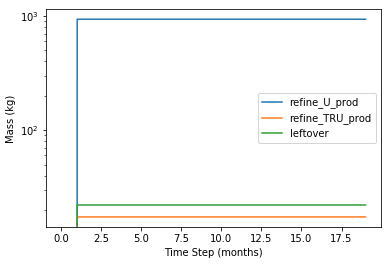
\includegraphics[width=\linewidth]{timeseries-prod}
			\caption{Product time series of a simple simulation.}
			\label{fig:timeseries-prod}
		\end{figure}
	\end{column}
	\begin{column}{.5\textwidth}
		\begin{figure}
			\centering
			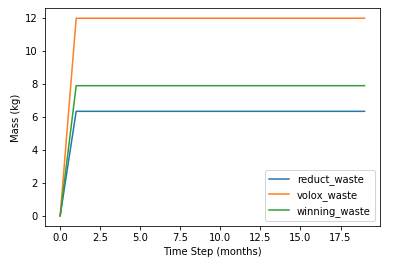
\includegraphics[width=\linewidth]{timeseries-waste}
			\caption{Waste time series of a simple simulation.}
			\label{fig:timeseries-waste}
		\end{figure}
	\end{column}
\end{columns} 
\end{frame}

\begin{frame}
\frametitle{Isotopic Composition of Waste Streams}
  \begin{figure}
  	\centering
  	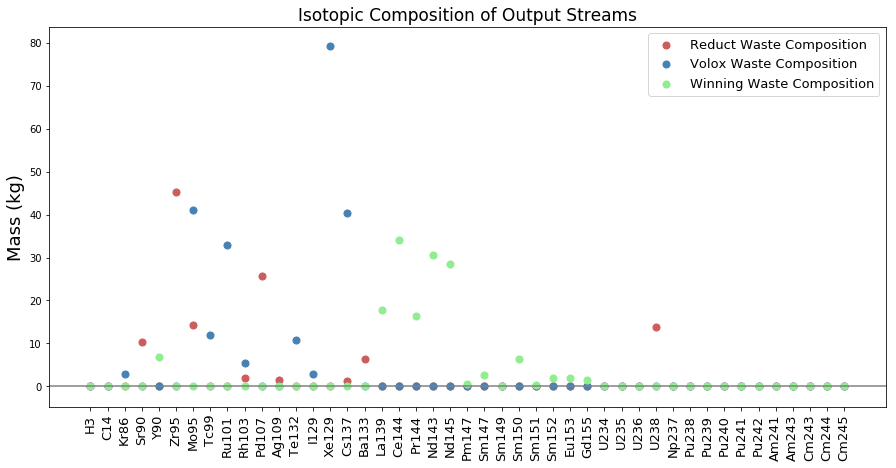
\includegraphics[width=0.9\linewidth]{avg-isotope-comp}
  	\caption{Isotopic Composition of Average Waste Streams}
  	\label{fig:avg-isotope-comp}
  \end{figure}
\end{frame}

\begin{frame}
\frametitle{Current Diversion}
  \begin{figure}
  	\centering
  	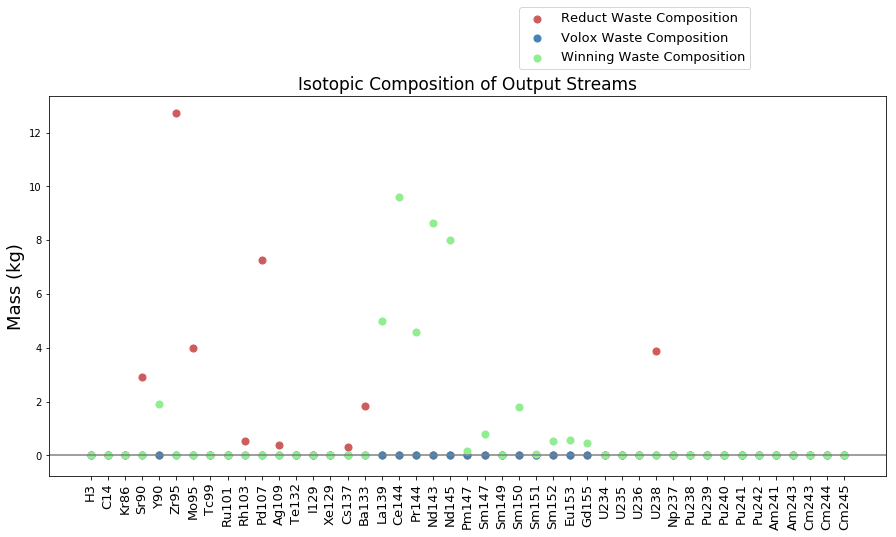
\includegraphics[width=0.9\linewidth]{current-isotope-comp}
  	\caption{Isotopic Composition of Current Diverted Waste Streams}
  	\label{fig:current-isotope-comp}
  \end{figure}
\end{frame}

\begin{frame}
  \frametitle{Isotopic Range}
  \begin{figure}
  	\centering
  	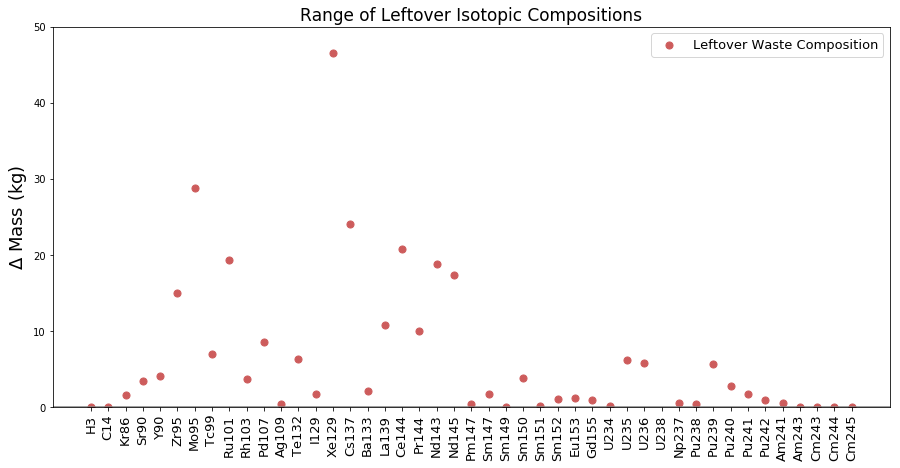
\includegraphics[width=0.9\linewidth]{isotopic-comp-range}
  	\caption{Range of Isotopic Values}
  	\label{fig:isotopic-range}
  \end{figure}
\end{frame}

